\subsection{Neural Networks}
In an artificial neural network, a neurone is a logistic unit, which is fed inputs through input wires. This unit can perform computations resulting in outputs that are transmitted through the output wires. An artificial neural network is simply a set of these logistic units strung together as shown in Figure~\ref{Fig:FigTwo}. Each two layers are connected together using weight parameters. As such, the neural network in Figure~\ref{Fig:FigTwo} possesses two weighting matrices, $\bm{\Theta}^{(1)}$ and $\bm{\Theta}^{(2)}$. Here, we used $\bm{\Theta}^{(l)}$ to denote the weights connecting layers $l$ and $l+1$. Definitely, the dimensionality of $\bm{\Theta}^{(l)}$ depends on the number of units in each of the two layers. For example, if layer $l$ consists of $s_{l}$ units and layer $l+1$ of $s_{l+1}$, $\bm{\Theta}^{(l)}$ has a dimensionality of $s_{l+1} \times s_{l} +1$, where we have added another dimension to incorporate the bias term (incorporated to increase the expressiveness of the functions learnt by the neural network). 

\begin{figure}[h!]
\label{Fig:FigTwo}
\centering 
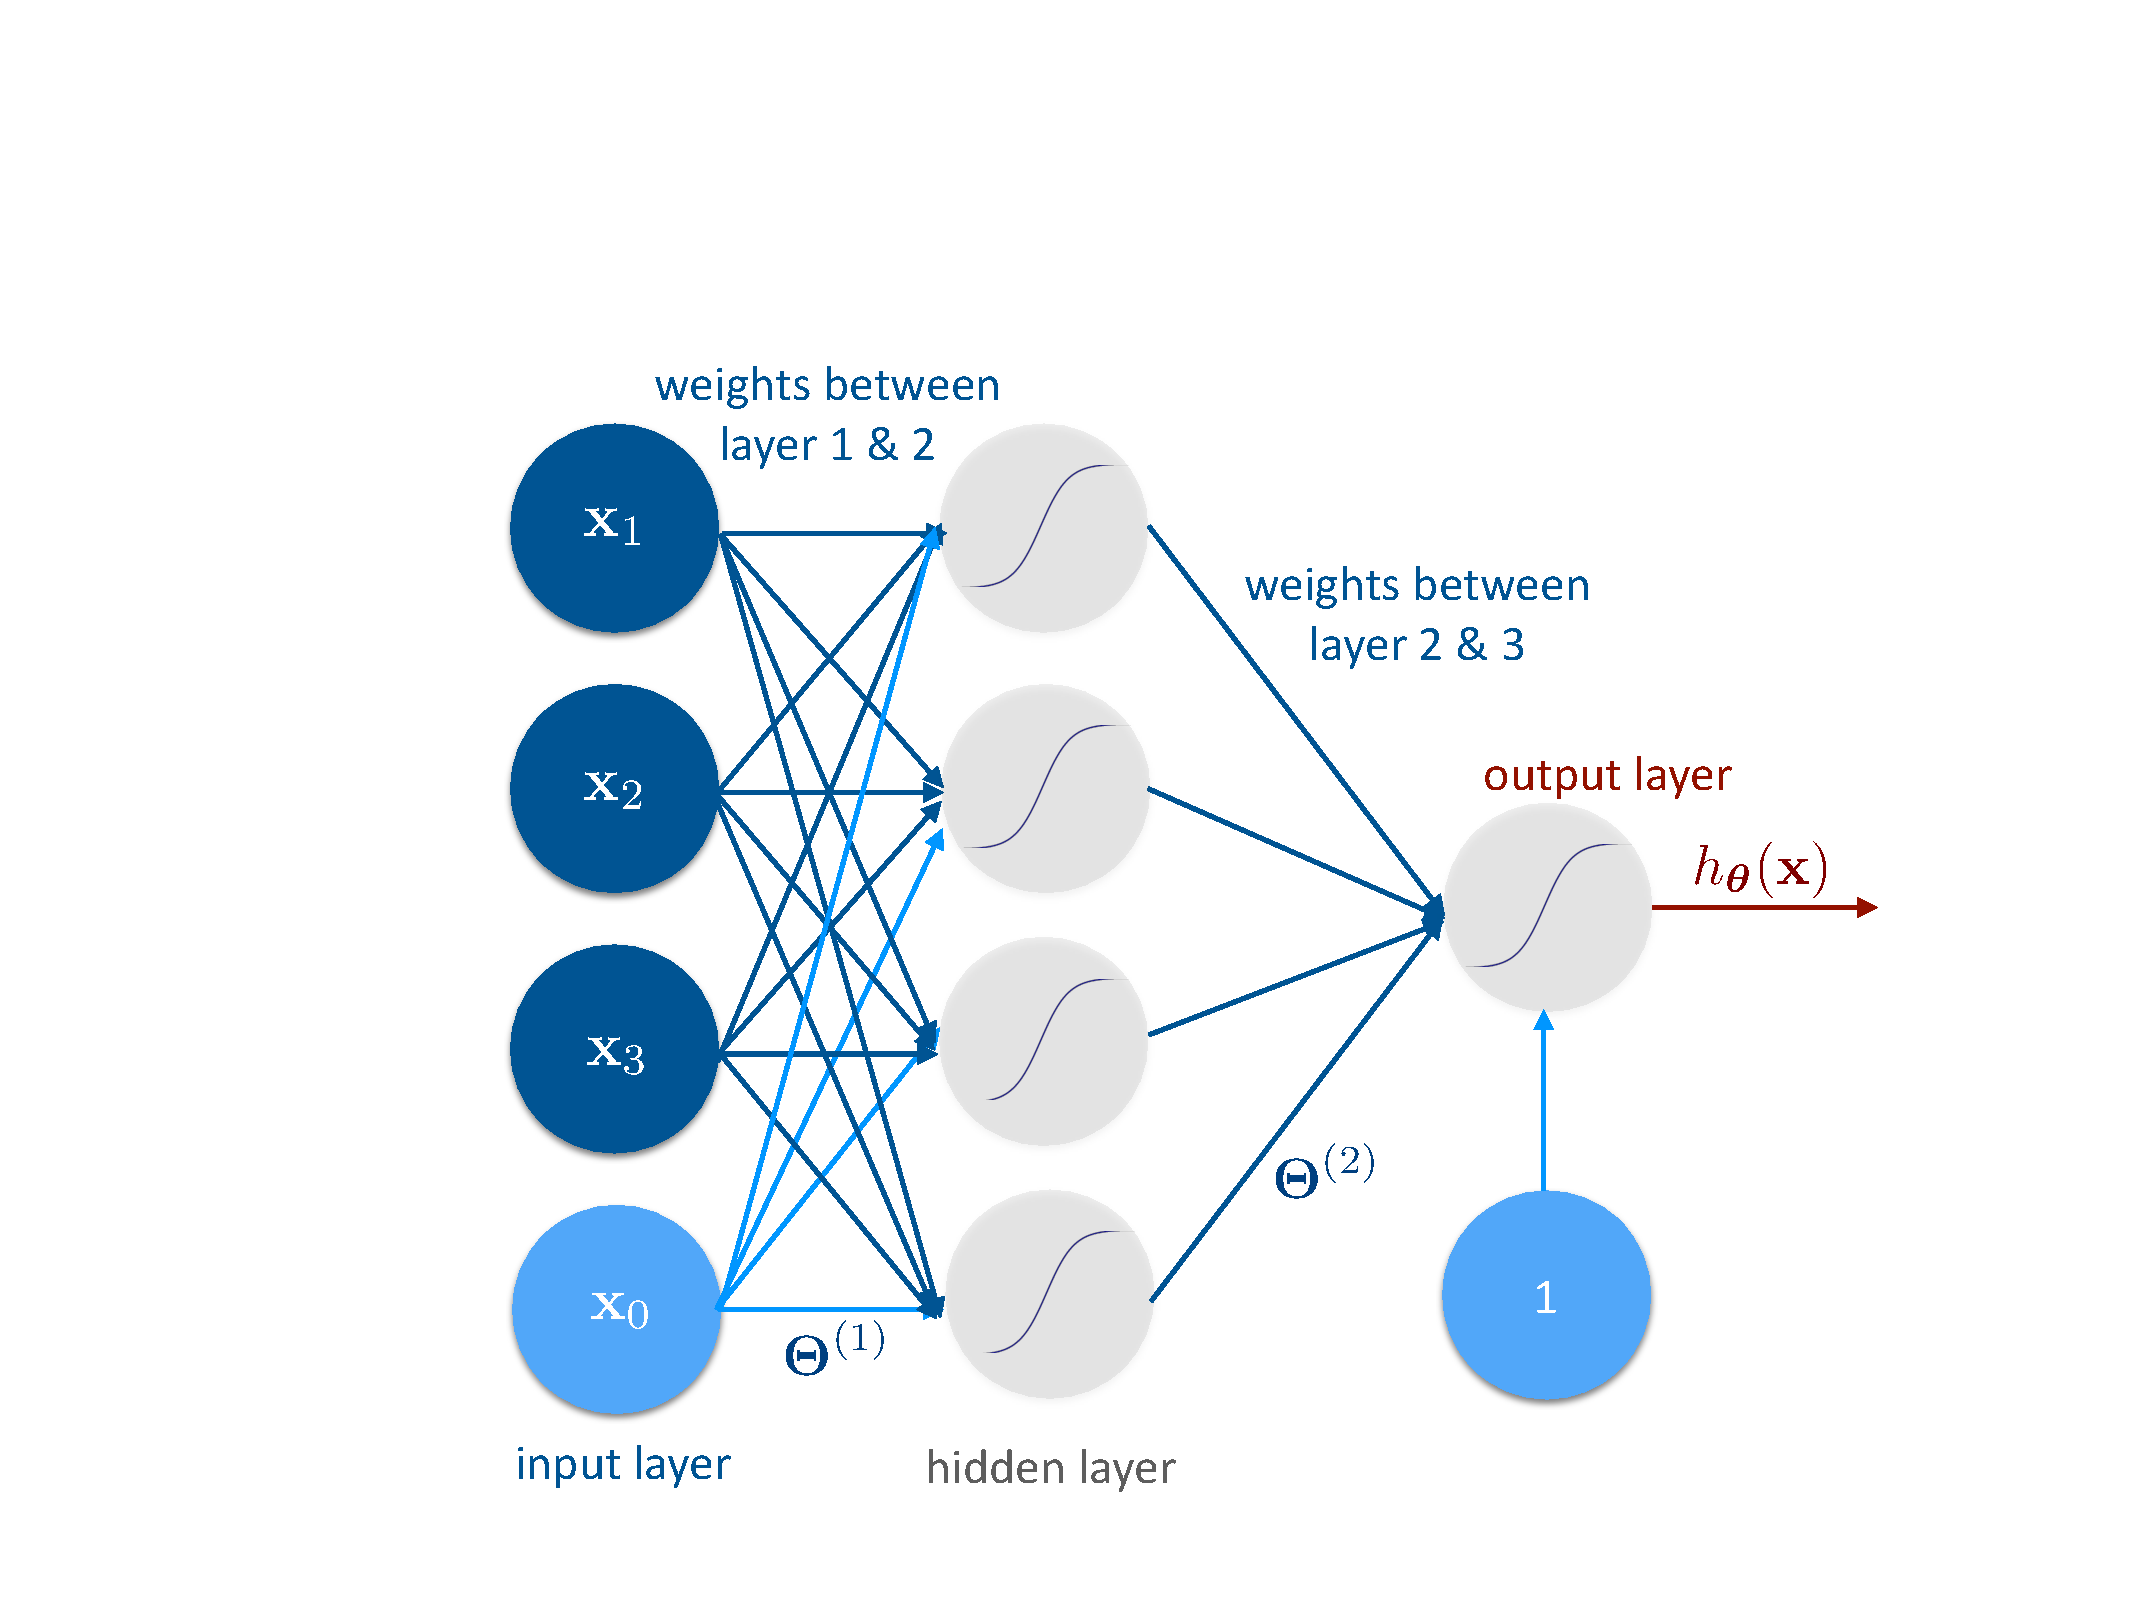
\includegraphics[trim = 10em 1em 10em 10em, clip, scale=.3]{NN}
\caption{A high-level depiction of an artificial neural network showing three layers as well as the weight connections between them.}
\end{figure}
\subsubsection{Feed Forward \& Feed Backward Propagation}
Given the notation introduced above, we are now ready to discuss the computations that are performed by a neural network. Intuitively, between every two layers the inputs from the previous layer are, first, linearly (through the weight matrices) propagated forward and then nonlinearly transformed (through the sigmoids) to produce an output on the successor layer. Recursing this process, which we refer to as forward propagation, over the total layers of the network will produce an output on the final layer $L$. 

\paragraph{Training \& Backward Propagation} Having described feed forward propagation, the next step is to detail the strategy by which neural networks determine the model parameters (i.e., the $\bm{\Theta}^{(l)}$ matrices). In standard regression or classification problems, back-propagation is the algorithm adopted. Given an input data point, back-propagation commences as follows. First, forward propagation is executed and the network is made to output a value. This value is then compared to the real output from the data set producing an error. This error is then propagated backwards to every other layer and used to update connecting weights. Such updates typically involve gradient-based methods (e.g., stochastic gradients). 